\documentclass[a4paper, 11pt]{amsart}
\usepackage{graphicx}
\usepackage[applemac]{inputenc}
%\usepackage[danish]{babel}
\usepackage{amssymb}
\usepackage{amsmath}
\usepackage{amsthm}
\usepackage{epstopdf}
\usepackage{fancyhdr}
%\usepackage{maplestd2e}


\numberwithin{equation}{section}

\pagestyle{fancy}
\chead{}
\lhead{}
\rhead{}
\DeclareGraphicsRule{.tif}{png}{.png}{`convert #1 `dirname #1`/`basename #1 .tif`.png}

\long\def\symbolfootnote[#1]#2{\begingroup%
\def\thefootnote{\fnsymbol{footnote}}\footnote[#1]{#2}\endgroup}

\renewcommand{\sectionmark}[1]{\markright{#1}{}}

\newcommand{\vek}[1]{\textbf{#1}}
\newcommand{\en}[1]{\;#1}
\newcommand{\enm}[1]{\;\textrm{$#1$}}
\newcommand{\pa}{\partial}
\newcommand{\ket}[1]{|#1\rangle}
\newcommand{\bra}[1]{\langle #1|}
\usepackage{float}
\usepackage{subfig}

\captionsetup{font=small, labelfont=bf}


\title{Statistical Methods for Machine Learning}
\author{Nicholas Clark \and Piotr Zywien \and Victor Yakimov}
\date{February $20^\mathrm{th}$, 2012}                                      
\fancyhead[L]{\textit{\nouppercase\rightmark}} 
\fancyhead[R]{\textit{Statistical Methods for Machine Learning}} 
\fancyfoot[C]{\thepage}
\def\maketitlepage{
	\thispagestyle{empty}
	\begin{center}
	\null
	\vskip 3cm
	\rule[15pt]{\textwidth}{1,5pt}
	{\LARGE \textbf{Statistical Methods for Machine Learning \Large \textit{\\[10pt]First Assignment}}}
	\\[18pt]
	\rule[15pt]{\textwidth}{1,5pt}
	\vskip 3cm
	\large \textbf{by:}\\[14pt]
	\large \textit{Nicholas Clark, Piotr Zywien, Victor Yakimov \\[2pt]
	}
	
	\end{center}
	}

\def\maketitleshart{
	\begin{flushright}
	{\LARGE \textbf{[Ttile]}}
	\\[4pt]
	\textit{[Authors - Date]}
	\end{flushright}
	\rule[10pt]{\textwidth}{1,5pt}
	\thispagestyle{plain}

	}

\usepackage{listings}
\usepackage[usenames,dvipsnames]{color}
\definecolor{lightgray}{rgb}{0.9,0.9,0.9}
\definecolor{darkgray}{rgb}{0.5,0.5,0.5}


\begin{document}
\begin{titlepage}
\maketitlepage
\end{titlepage}
\newpage
% \tableofcontents %we don't need no stinking table of contents
\newpage
\section*{Readme}

\lstloadlanguages{R} 

\lstset{% general command to set parameter(s)
language=R,
basicstyle=\scriptsize \ttfamily,
commentstyle=\ttfamily \color{darkgray},
numbers=left,
numberstyle=\ttfamily \color{darkgray} \footnotesize,
stepnumber=1,
numbersep=5pt,
backgroundcolor=\color{lightgray},
showspaces=false,
showstringspaces=false,
showtabs=false,
frame=single,
tabsize=2,
captionpos=b,
breaklines=true,
breakatwhitespace=false,
title=\lstname,
escapeinside={},
keywordstyle={},
morekeywords={}}

All the code has been run and tested in \texttt{R 2.13.1} using \texttt{RStudio 0.94.110} on an Apple x86\_64, darwin9.8.0 system. Packages required are \texttt{pixmap}, \texttt{ggplot2}, and \texttt{gplots}. A current version of \texttt{R} can be obtained directly from CRAN's website, \texttt{http://cran.r-project.org}, and packages can be installed from the CRAN repository by running the command \texttt{install.packages} from the \texttt{R} environment. Also

\section*{Question 1}
The normal distribution with parameters $\mu,\sigma=(-1,1),(0,2),(2,3)$ can be seen in figure \ref{1dgauss}.
\begin{figure}[h!]
  \centering
\includegraphics[width=0.32\textwidth]{1dgauss11}
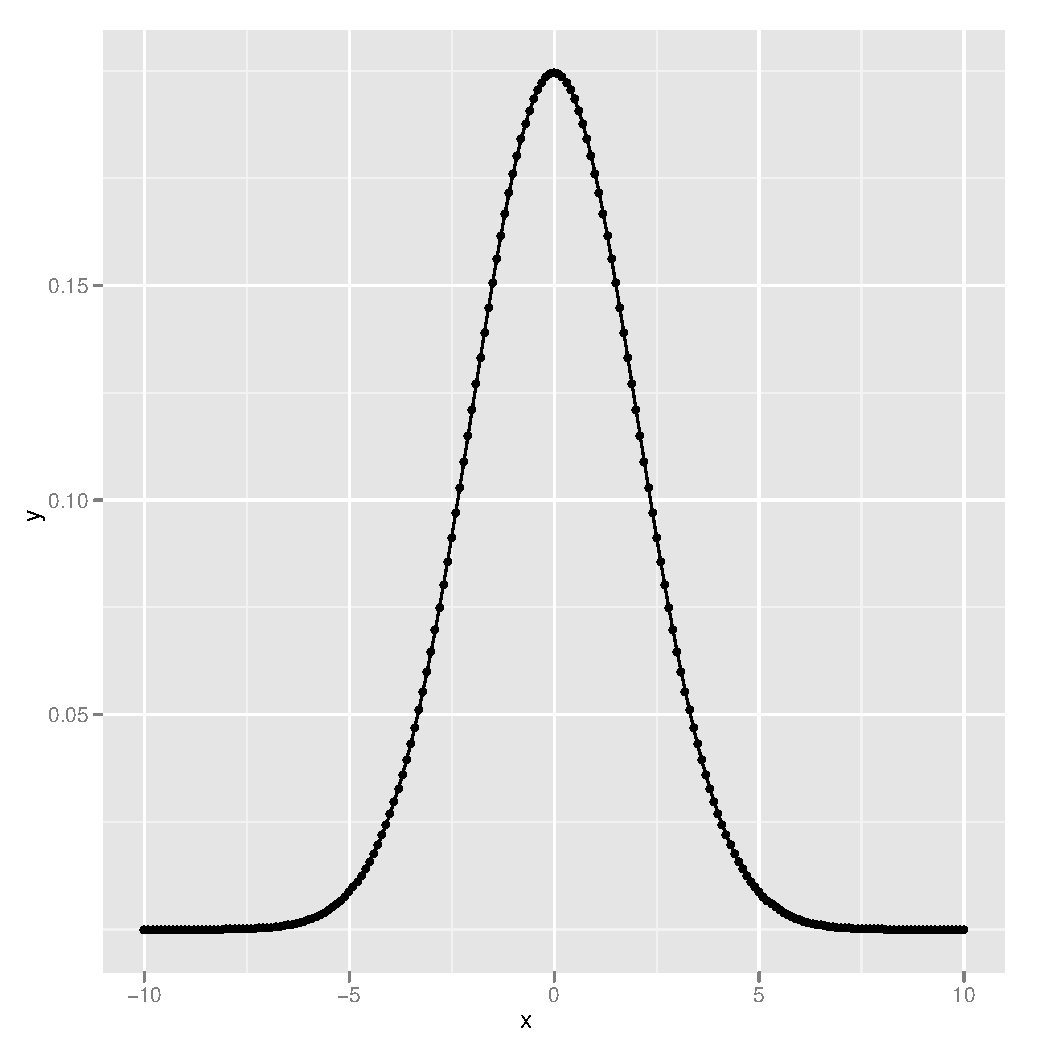
\includegraphics[width=0.32\textwidth]{1dgauss02}
\includegraphics[width=0.32\textwidth]{1dgauss23}
\caption{Gaussian distributions with $\mu,\sigma=(-1,1),(0,2),(2,3)$}
\label{1dgauss}
\end{figure}

\section*{Question 2}
In figure \ref{samps} we have two empirical plots of a 2-dimensional gaussian, with $\mu=(1,1)^T$ and $\sigma=\left[\begin{array}{cc}0.3 & 0.2 \\0.2 & 0.2\end{array}\right]$. One has a sample size N = 100, and the other a sample size N = 10000, with binned counts shown as a heat-map. 

\begin{figure}[h!]
  \centering
\includegraphics[width=0.45\textwidth]{2dgauss100}
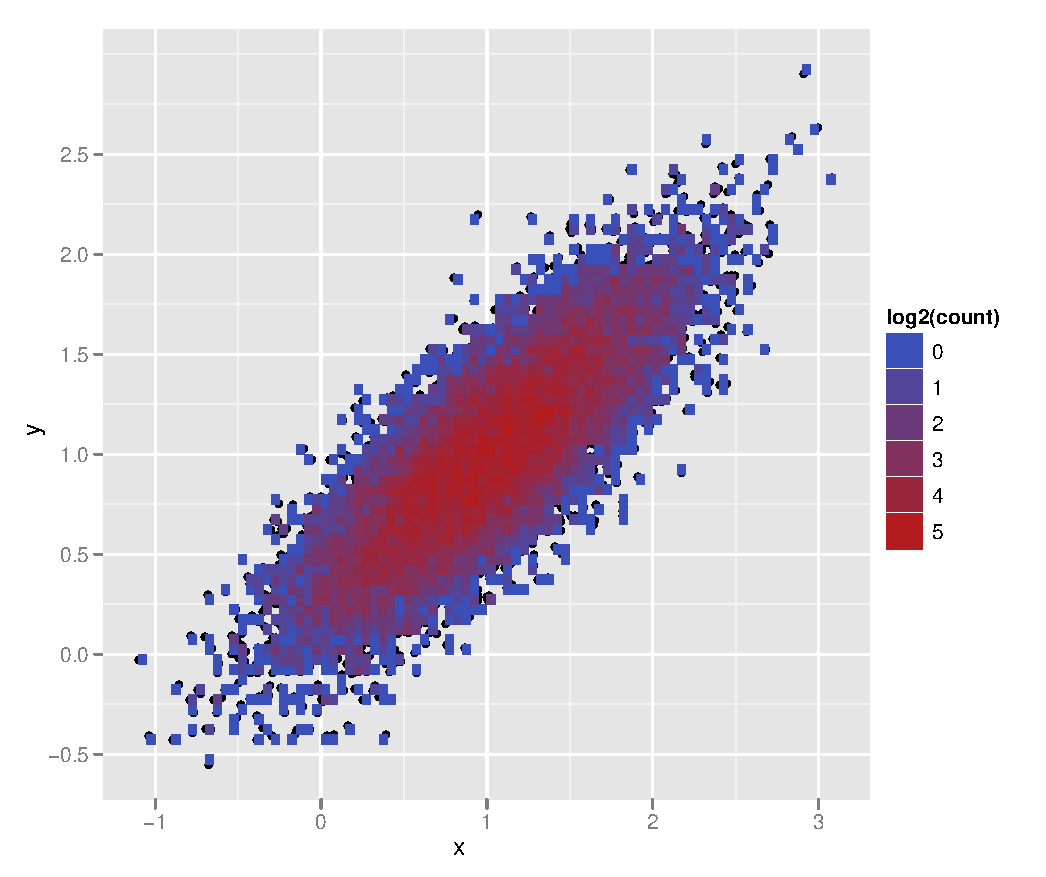
\includegraphics[width=0.45\textwidth]{2dgauss10k}
\caption{One hundred samples drawn from a 2-dimensional gaussian, and one hundred thousand samples drawn from a 2-dimensional gaussian with binned counts, drawn for comparison}
\label{samps}
\end{figure}


\section*{Question 3}
The sample mean and covariance is $\mu_{ML}=(1.076,1.065)^T$ and $\Sigma_{ML}=\left[\begin{array}{cc}0.340 & 0.225 \\0.225 & 0.210\end{array}\right]$. The sample mean and the correct mean can be seen on figure \ref{sampmean}. The two differ, as the samples drawn from a gaussian are naturally stochastic. The sample mean and the true mean will converge as the sample number $N\rightarrow\infty$. In our case the sample mean deviates by $(0.076,0.065)$ from the true mean

\begin{figure}[h!]
  \centering
\includegraphics[width=0.7\textwidth]{2dmuml}
\caption{One hundred samples drawn from a 2d-gaussian distribution. The blue dot represents the true mean of the distribution used, and the red dot represents the sample mean}
\label{sampmean}
\end{figure}

\section*{Question 4}
In order to show an expression of conditional trivariate Gaussian distribution, $p(x_a|x_b)$ with $x_c$ marginalized out,  we use formula (2.97) from Bishop:
%\begin{equation}
\[
\mu_{a�b}=\mu_a-\Lambda_{aa}^{-1}\Lambda_{ab}(x_b-\mu_b) %\Leftrightarrow
\]
%\end{equation}
and equations (2.79)
%\begin{equation}
\[
\Lambda_{aa}=(\Sigma_{aa}-\Sigma_{ab}\Sigma_{bb}^{-1}\Sigma_{ba})^{-1}
\]
%\end{equation}
and (2.80)
\[
\Lambda_{ab}=-(\Sigma_{aa}-\Sigma_{ab}\Sigma_{bb}^{-1}\Sigma_{ba})^{-1}\Sigma_{ab}\Sigma_{bb}^{-1}
\]
Insertion gives
\[
\mu_{a�b}=\mu_a-(\Sigma_{aa}-\Sigma_{ab}\Sigma_{bb}^{-1}\Sigma_{ba})(-(\Sigma_{aa}-\Sigma_{ab}\Sigma_{bb}^{-1}\Sigma_{ba})^{-1}\Sigma_{ab}\Sigma_{bb}^{-1})(x_b-\mu_b)
\]
\[
\Leftrightarrow \mu_{a�b}=\mu_a+\Sigma_{ab}\Sigma_{bb}^{-1}(x_b-\mu_b)
\]
And by equation 2.79, $\Lambda^{-1}_{aa}= \Sigma_{aa}-\Sigma_{ab}\Sigma_{bb}^{-1}\Sigma_{ba}$. We can insert those values into $p(x_a|x_b)=\mathcal{N}(x|\mu_{a|b},\Lambda_{aa}^{-1})$
\section*{Question 5}

As is apparent from figure \ref{px1hist}, large bins result in a loss of detail (as is the case with 5 bins in the figure), while small bins can often be misleading as they are too sensitive to outliers (as is the case with 100 bins). 
\begin{figure}[h!]
  \centering
\includegraphics[width=0.24\textwidth]{px1hist100}
\includegraphics[width=0.24\textwidth]{px1hist25}
\includegraphics[width=0.24\textwidth]{px1hist10}
\includegraphics[width=0.24\textwidth]{px1hist5}
\includegraphics[width=0.24\textwidth]{px2hist100}
\includegraphics[width=0.24\textwidth]{px2hist25}
\includegraphics[width=0.24\textwidth]{px2hist10}
\includegraphics[width=0.24\textwidth]{px2hist5}
\caption{The first dimension $p(x_1)$ (top row) and second dimension $p(x_2)$ (bottom row) of one hundred samples from a 2-dimensional gaussian represented as a histogram, with different bin widths. The number of bins is 100, 25, 10 and 5, per column }
\label{px1hist}
\end{figure}


\section*{Question 6}

The histogram for the first dimension $p(x_1)$ of one hundred samples from a 2-dimensional gaussian, plotted along with its analytical solution, with $\mu=1$, $\sigma=0.3$ shown in figure \ref{px1histanal}. The analytical expression for the marginal distribution $p(x_1)$ is \[\mathcal{N}(\mu=\mu_1,\sigma^2=\sigma^2_{11})=\frac{1}{\sigma \sqrt{2 \pi} } e^{-\frac{(x-\mu)^2}{2\sigma^2}}\] given a bivariate Gaussian with $\mu=(\mu_1,\mu_2)^T$ and $\Sigma=\left[\begin{array}{cc}\sigma_{11} & \sigma_{12} \\\sigma_{21} & \sigma_{22}\end{array}\right]$


\begin{figure}[h!]
  \centering
\includegraphics[width=1.00\textwidth]{px1histanal}
\caption{The first dimension $p(x_1)$ of one hundred samples from a 2-dimensional gaussian represented as a histogram, plotted along with the analytical solution for the mean and covariance parameters.}
\label{px1histanal}
\end{figure}
\section*{Question 7}
In figure \ref{2dhist} we show 2-dimensional histogram estimate of p(x), using 100,1000,10000 samples and $10\times 10$, $15\times 15$, and $20 \times 20$ bins. Larger number of samples mean we can decrease the bin-width further and provide more resolution of the histogram. Histograms with small bin sizes and few samples tend to behave more erratically -- i.e. if we were to replot all the histograms, the one with the least samples and smallest bins would vary most.

\begin{figure}[h!]
  \centering
\includegraphics[width=0.32\textwidth]{twodhist1}
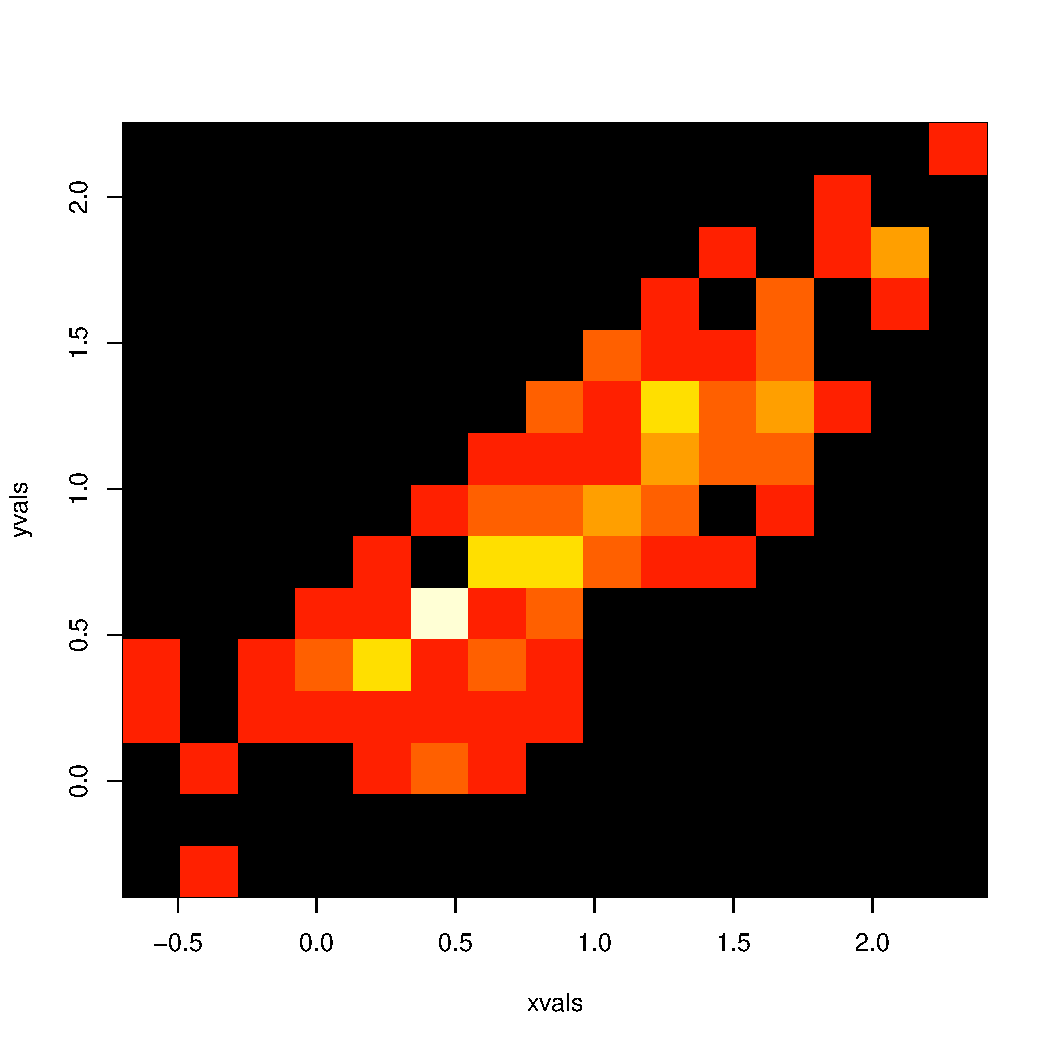
\includegraphics[width=0.32\textwidth]{twodhist2}
\includegraphics[width=0.32\textwidth]{twodhist3}
\includegraphics[width=0.32\textwidth]{twodhist4}
\includegraphics[width=0.32\textwidth]{twodhist5}
\includegraphics[width=0.32\textwidth]{twodhist6}
\includegraphics[width=0.32\textwidth]{twodhist7}
\includegraphics[width=0.32\textwidth]{twodhist8}
\includegraphics[width=0.32\textwidth]{twodhist9}
\caption{2D-histograms. First row contains 100 samples, second row contains 1000 samples, and the third row contains 10000 samples. The first column has $10\times10$ bins, the second $15\times15$ bins, and the third $20\times20$ bins}
\label{2dhist}
\end{figure}
\section*{Question 8}
We derive a function $h(z)=1/\lambda \cdot \ln{(1-z)}$ which is the integral of $p(y)$.  We then generate a uniformly random number $z \in [0,1]$ L=10,100,1000 times which we use to estimate $\mu$ of $p(y)$. Repeating the estimation 1000 times, we get a gaussian distribution of means, as predicted by the central limit theorem. A normal quantile-quantile plot, as well as a histogram of the means,  shown in figure \ref{q} shows that a thousand means drawn from L=1000,100,10 very closely approximate a Gaussian distribution, centered around the true mean of $\mu=1/\lambda=1/3$. We get a standard deviation of the mean of $\sigma=0.104$, $\sigma= 0.0324$, and $\sigma=0.0108$ for L=1000, L=100, and L=10,  respectively.
\begin{figure}[h!]
  \centering
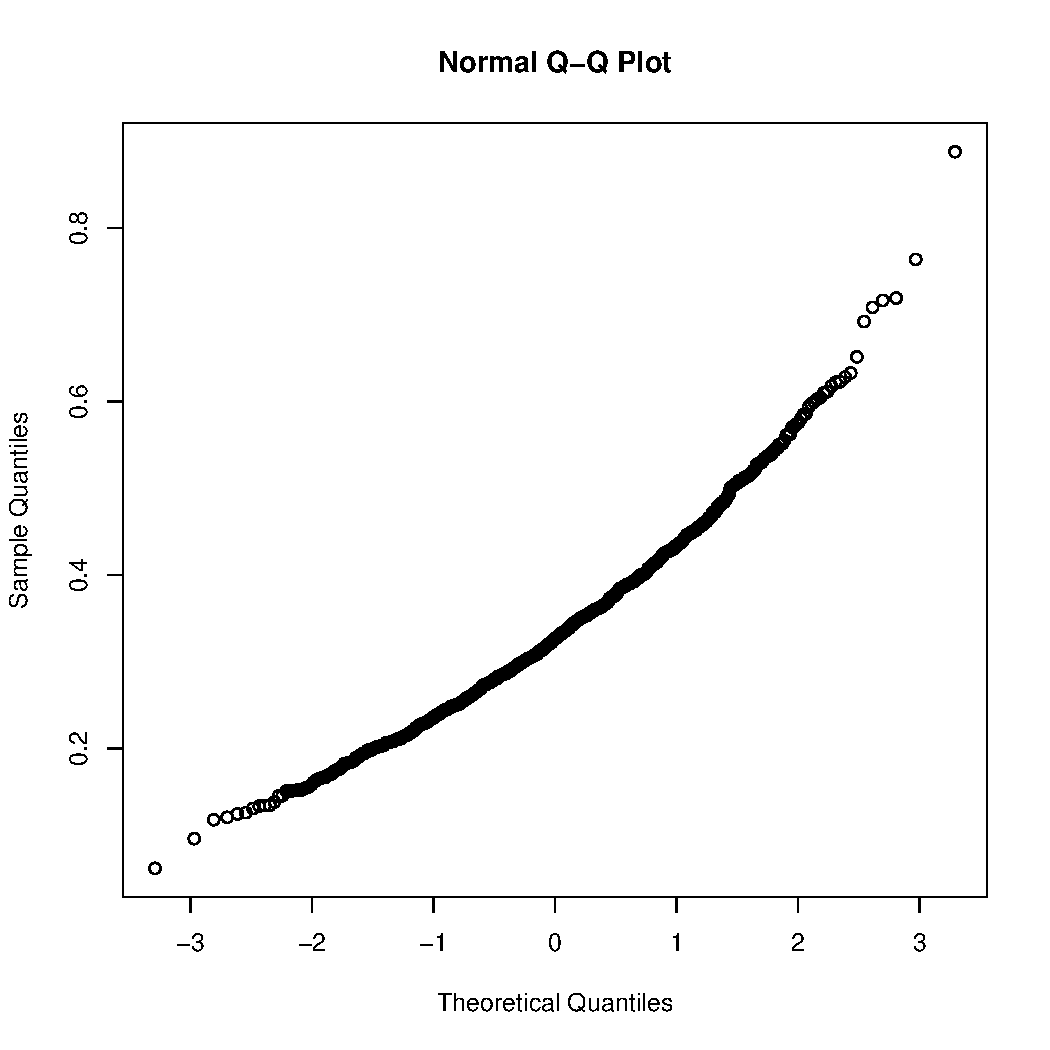
\includegraphics[width=0.45\textwidth]{qqplot1}
\includegraphics[width=0.45\textwidth]{normeans1}
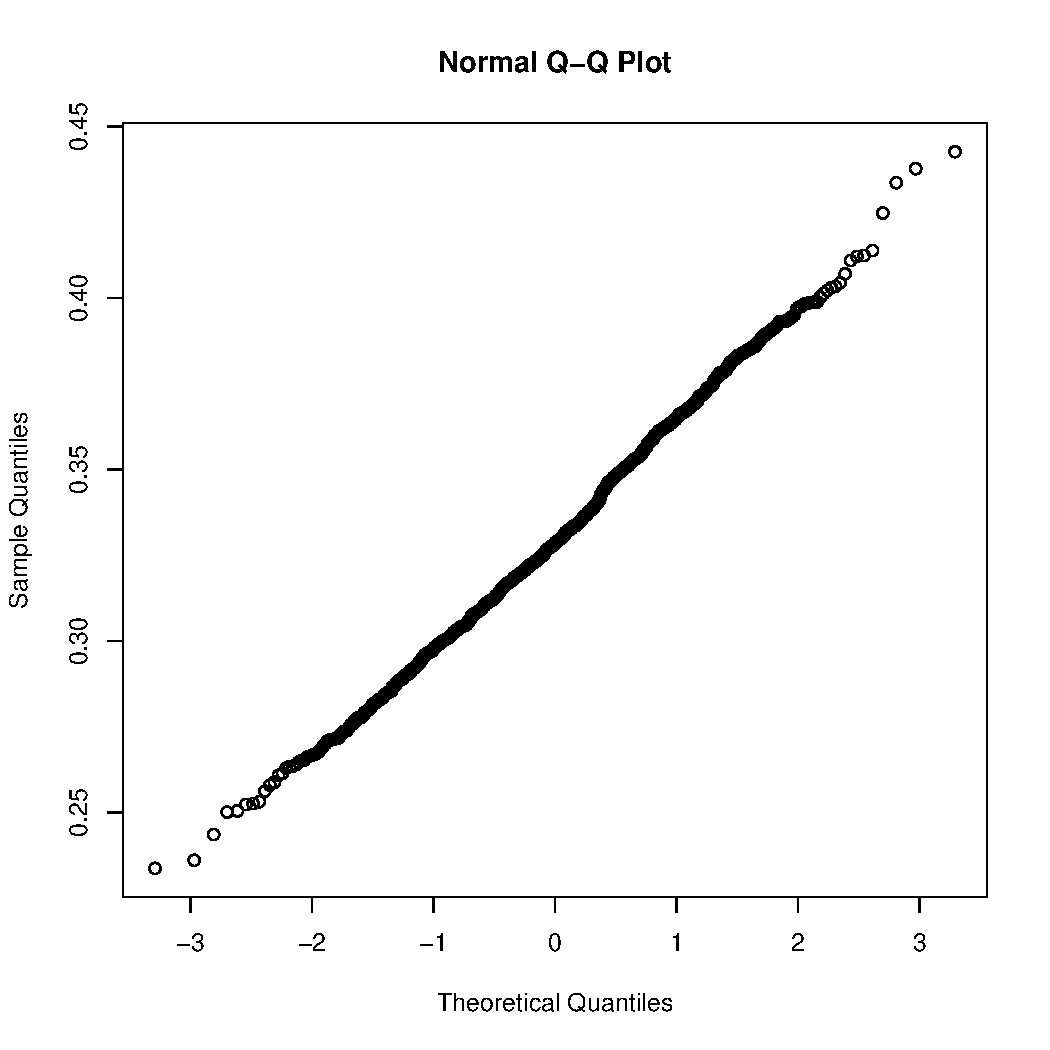
\includegraphics[width=0.45\textwidth]{qqplot2}
\includegraphics[width=0.45\textwidth]{normeans2}
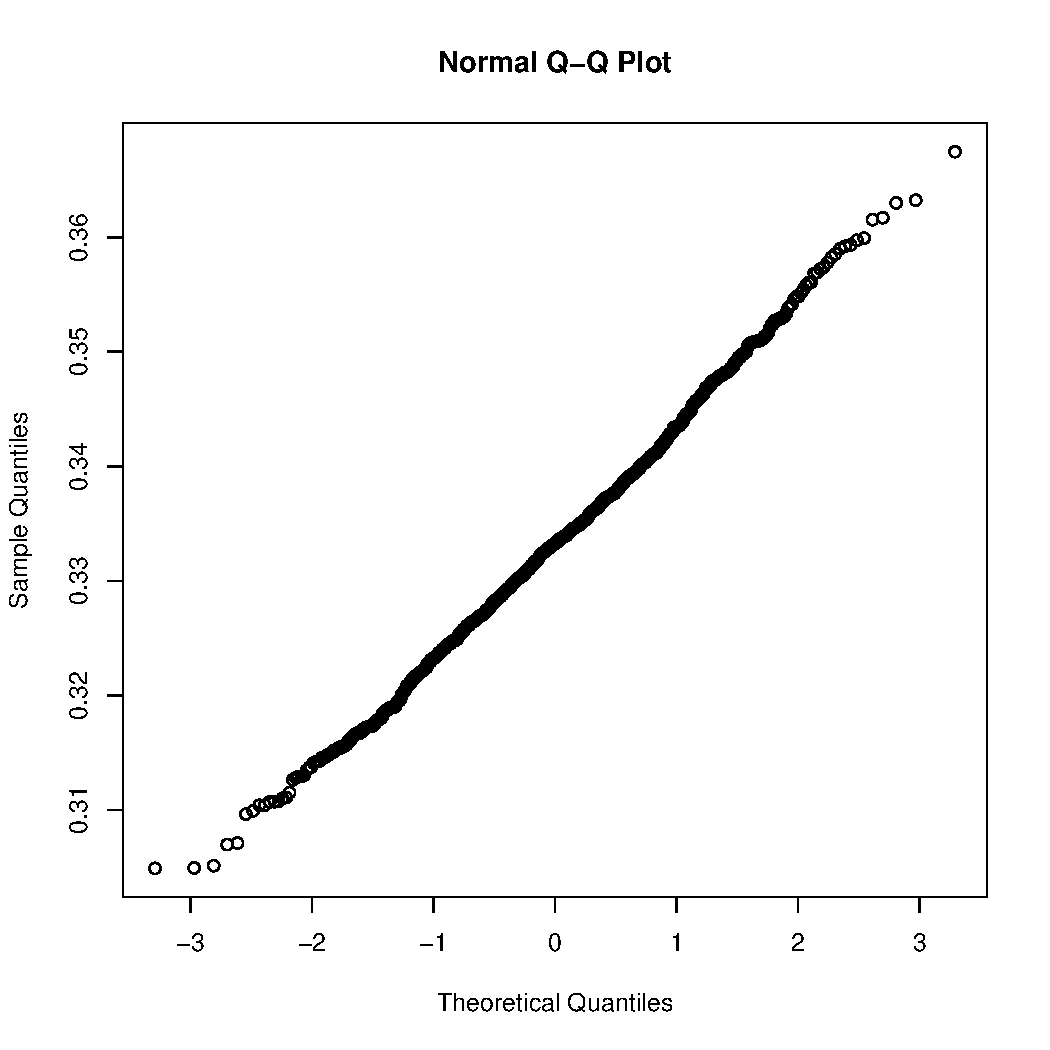
\includegraphics[width=0.45\textwidth]{qqplot3}
\includegraphics[width=0.45\textwidth]{normeans3}
\caption{Quantile-quantile plot and histogram for the distribution of $\mu$ with L=10,100,1000, shown in rows 1, 2, and 3}
\label{q}
\end{figure}

We also show in figure \ref{deviation} how the sample mean deviates from the true mean with varying values of L sizes. In general, for all three values of L, the sample mean should be around the true mean, with the only difference being the variance of means.
\begin{figure}[h!]
  \centering
\includegraphics[width=1.00\textwidth]{deviation}
\caption{The deviation from the true mean with increasing L}
\label{deviation}
\end{figure}

A transformation of the expected absolute deviation, when plotted against L will produce a straight line, given the transformation is the inverse of the square of said mean absolute deviation.
Thus, the plotted points will be as such: ( 10, $\frac{1}{mad( means1 )^2}$ ), ( 100, $\frac{1}{mad( means2 )^2}$ ) and ( 1000, $\frac{1}{mad( means3 )^2}$ ), where mad is the mean absolute deviation function and means1, means2 and means3 are mean values plotted in figure \ref{q}. The straight plotted line is shown in figure \ref{madstraight}. This reflects the property that in order to achieve higher precision equivalent to the square root of the standard deviation, the amount of data has to be proportionally increased by a factor of 10.

\begin{figure}[h!]
  \centering
\includegraphics[width=1.00\textwidth]{madstraight}
\caption{Plot of the inverse squares marginal average distributions of means against L, where L is 10, 100 and 1000}
\label{madstraight}
\end{figure}

\section*{Question 9}
The red pitcher is detected with remarkable accuracy, and the probability density is shown in figure \ref{pitcher}.
\begin{figure}[h!]
  \centering
\includegraphics[width=0.49\textwidth]{pitcher}
\includegraphics[width=0.49\textwidth]{centerOfMass}
\caption{ probability density of pitcher detection, along with its center of mass }
\label{pitcher}
\end{figure}
The pitcher is detected, and no pixels from outside the pitcher are picked up. Specular highlights present in the center of the image are not detected as they do not have the same color distribution as the training set --- the training set is mostly red, and the specular highlights are mostly white. 

\section*{Question 10}
The center of mass can be seen in figure \ref{pitcher} and the iso-probability curves along with the spatial covariance are shown in figure \ref{spat}. 

\begin{figure}[h!]
  \centering
\includegraphics[width=0.45\textwidth]{spat}
\includegraphics[width=0.45\textwidth]{newMap}
\caption{ iso-probability curves and 2-d probabilities for kande2.png}
\label{spat}
\end{figure}

\section*{Question 11}
We test our trained model on a different picture of a pitcher. We use the same training data, and display the probability that pixels from the new image are a part of the old distribution. We get the 2-d probability map shown in figure \ref{spat}. The results are poor, which is unsurprising as the pitcher appears as a significantly different shade of red under the different lighting conditions. 


\end{document}